\section{Gestion de projet}
\subsection{Equipe de développement}
Au début du projet, nous avons essayer de déterminer des rôles et les tâches qui y sont attachées.

Nous avons déterminés les rôles suivant :
\begin{itemize}
 \item Un chef de projet, dont le rôle principal est d'assurer la coordination de l'équipe~;
 \item Un architecte, chargé de concevoir l'organisation du framework~;
 \item Un dévelopeur, en charge d'implémenter notre solution~;
 \item Un responsable qualité, en charge d'assurer la qualité du produit et sa validité.
\end{itemize}
Le détail de ces reponsabilités est décrit dans la figure \ref{fig:repart_effect} p.\pageref{fig:repart_effect}, partie "Rôles modélisés".

Il est apparu que ces rôles n'étaient pas applicable en raison de leur poids différents, d'une part, mais aussi des compétences et aspirations de chacun. Nous avons éstimé la répartition des tâches comme décrit figure \ref{fig:repart_effect} p.\pageref{fig:repart_effect} partie "Rôles prévus".
La répartition effective est également décrite.

\subsection{Répartition des tâches}
\begin{figure}[thbp]
	\centering
		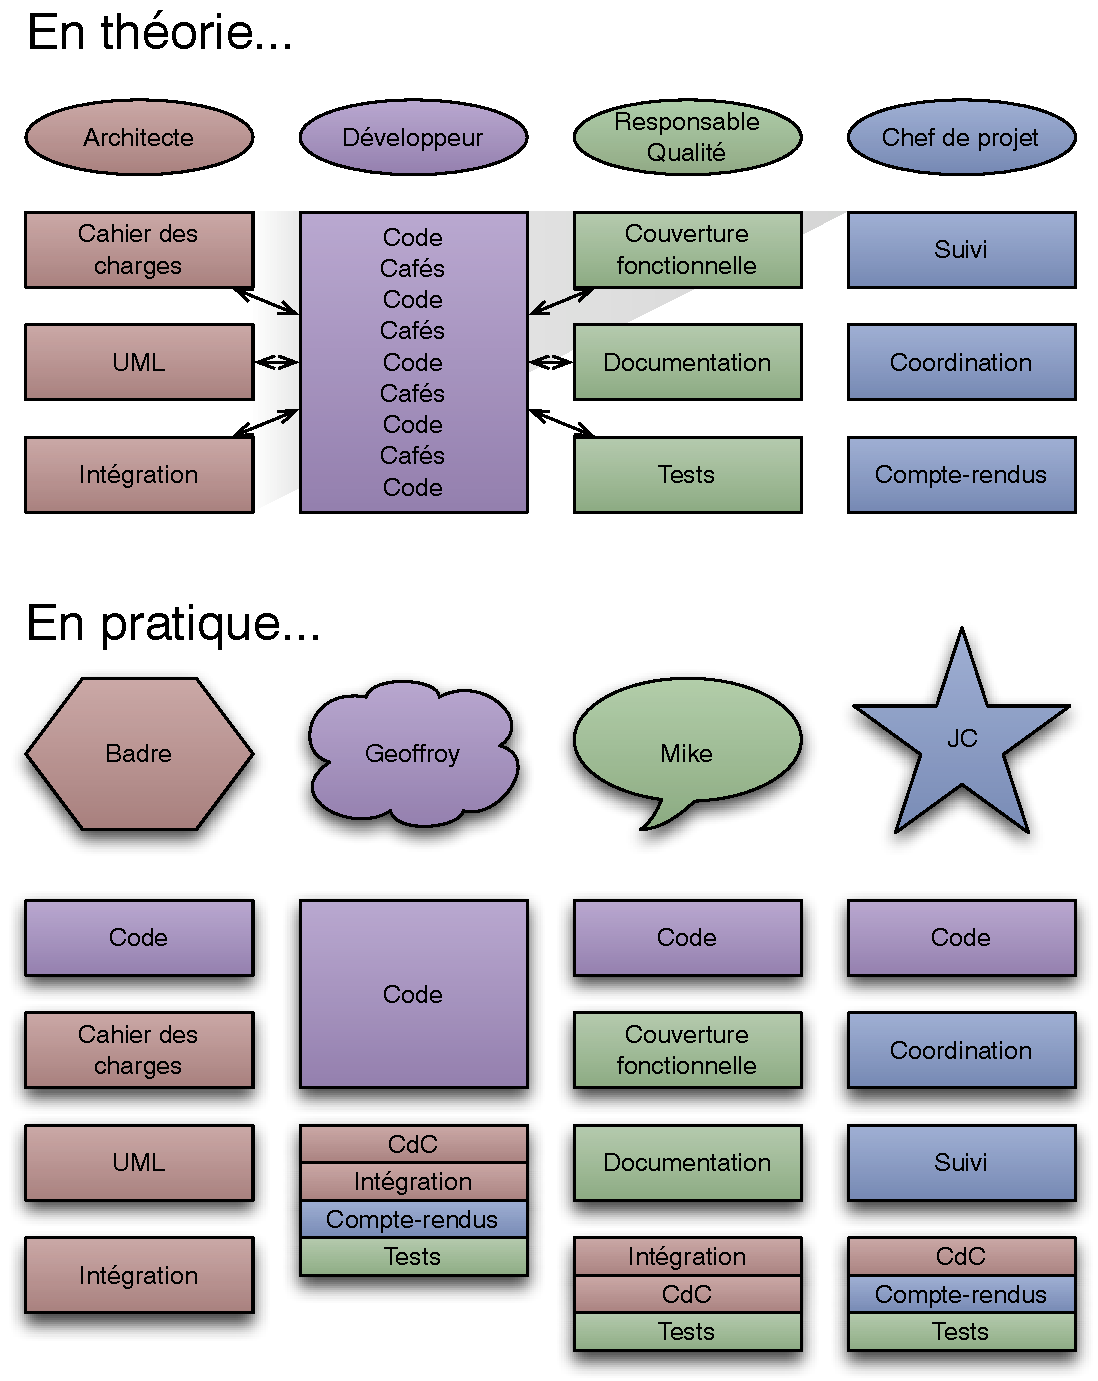
\includegraphics[angle=90, scale=0.7]{../diagrammes/repartition_taches.pdf}
	\caption{Répartition effective}
	\label{fig:repart_effect}
\end{figure}
\subsubsection{Prévisionnelle}

Cette répartition, a été choisie et acceptée par chacun des membres de l'équipe de développement.
Ainsi chaque membre de l'équipe a pu choisir d'assummer les fonctions en fonction des ses motivations et compétences.

\subsubsection{Effective}

La répartition prévisionelle des tâches n'a pas été entierrement respectée durant la réalisation du projet.
En effet, notre équipe a dû adapter la mobilisation de ses ressources pour s'adapter aux besoins du projet.

\subsection{Organisation du travail}
\begin{figure}[thbp]
	\centering
		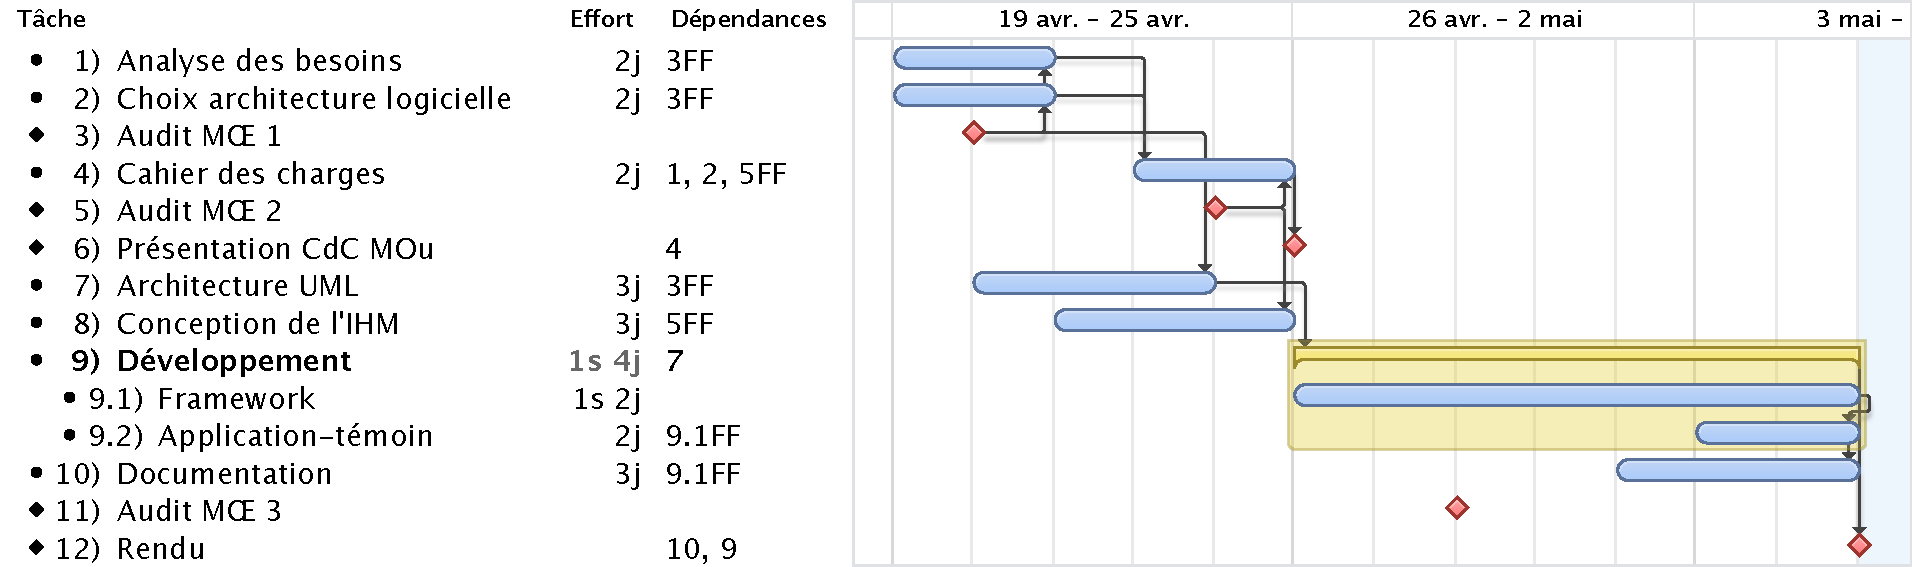
\includegraphics[angle=90, scale=0.7]{../diagrammes/gantt_final.pdf}
	\caption{Diagramme de Gantt}
	\label{fig:gantt}
\end{figure}

Après avoir determiné le temps et le nombre de ressources que nous pouvions nous permettre d'utiliser pour chaque tâche, un diagramme de gantt a pu être crée. Voir figure  \ref{fig:gantt} p.\pageref{fig:gantt}